\documentclass[12pt,a4paper]{article} 

\usepackage{fn2kursstyle}
\usepackage[russian]{babel}
\usepackage[T2A]{fontenc} 
\usepackage[utf8]{inputenc} 
\usepackage{geometry}
\usepackage{mathtools}
\usepackage{tikz}
\usepackage{chngcntr}

\counterwithout{equation}{section}
\counterwithout{figure}{section}
\frenchspacing 

\makeatletter
\newcommand*{\rom}[1]{\expandafter\@slowromancap\romannumeral #1@}
\makeatother

\title{Модель двух конкурирующих видов}
\group{ФН2-42Б}
\author{А.\,И.~Токарев}
\supervisor{М.\,П.~Галанин}
\date{2021}

\newcommand*\circled[1]{\tikz[baseline=(char.base)]{
            \node[shape=circle,draw,inner sep=2pt] (char) {#1};}}

\makeatletter
\newenvironment{sqcases}{%
  \matrix@check\sqcases\env@sqcases
}{%
  \endarray\right.%
}
\def\env@sqcases{%
  \let\@ifnextchar\new@ifnextchar
  \left\lbrack
  \def\arraystretch{1.2}%
  \array{@{}l@{\quad}l@{}}%
}
\makeatother

\begin{document}
    \maketitle
    \tableofcontents
    \pagebreak

    \section-{Введение}
    В теории, если нет никаких факторов воздействия внешней среды на некоторую популяцию, то она способна размножаться вплоть до бесконечности. Однако в реальной жизни так не происходит, и особи разных видов так или иначе воздействуют друг на друга. И одним из таких типов взаимодействий является конкуренция. Ее разделяют на внутривидовую конкуренцию (соперничество между особями одного вида за жизненные ресурсы) и на межвидовую конкуренцию (взаимоотношение между популяциями двух (или более) видов, которое неблагоприятно сказывается на их росте и выживании). 

    Проблема динамики популяции заинтересовала ученых еще в \rom{18} веке. Именно тогда они начали заниматься разработкой методов, способных описать динамику роста и сокращения популяций живых организмов.
    
    Основателем современной математической теории популяций справедливо считается Вито Вольтерра\footnote{В.\,Вольтерра (\textit{ит.} Vito Volterra, 1860--1940) --- итальянский математик и физик.}, разработавший математическую теорию биологических сообществ, аппаратом которой служат дифференциальные и интегро-дифференциальные уравнения. Эта модель основывается на следующих гипотезах:
    \begin{enumerate}
        \item Пища имеется в неограниченном количестве или ее поступление регулируется;
        \item В единицу времени погибает одинаковое количество особей одного вида;
        \item Прирост численности вида пропорционален его текущей численности.
    \end{enumerate}

    \section{Постановка задачи}
    Рассмотрим задачу из области динамики популяций. Пусть есть два сходных вида, конкурирующих между собой за пищу. Очевидно, что возможны следующие варианты: 
    \pagebreak
    \begin{itemize}
        \item Выживает только первый вид;
        \item Выживает только второй вид;
        \item Выживают оба вида;
        \item Оба вида вымирают.
    \end{itemize}
    
    Каждый из этих вариантов соответствует наличию своего положения равновесия. Тем самым для описания данной системы нужна модель с четырьмя стационарными точками --- стационарными состояниями системы.

    В соответствии с гипотезами В.\,Вольтерра модель двух конкурирующих видов выглядит следующим образом:
    \begin{equation}
        \label{volterra}
        \begin{cases}
            \frac{dx_1}{dt} = a_1 x_1 - b_{12} x_1 x_2 - c_1 {x_1}\!^2,
            \\
            \frac{dx_2}{dt} = a_2 x_2 - b_{21} x_2 x_1 - c_2 {x_2}\!^2 ,
        \end{cases}
    \end{equation}
    \noindent где $a_1, a_2$ --- коэфициенты скорости роста популяции; $b_{12}, b_{21}$ --- коэфициенты межвидовой борьбы; $c_1, c_2$ --- внутривидовой борьбы первого и второго вида соответсвенно.

    В данной курсовой работе необходимо рассмотреть все варианты параметров системы и исследовать качественное поведение ее решений. Также важно уделить внимание особым точкам системы.

    \section{Стационарные состояния}

    Найдем стационарные точки. Для этого необходимо решить систему уравнений вида: 
    \begin{equation}
        \label{seps}
        \begin{cases}
            a_1 x_1 - b_{12} x_1 x_2 - c_1 {x_1}\!^2 = x_1 (a_1 - b_{12} x_2 - c_1 x_1) = 0,
            \\
            a_2 x_2 - b_{21} x_2 x_1 - c_2 {x_2}\!^2 = x_2 (a_2 - b_{21} x_1 - c_2 x_2) = 0,
        \end{cases}
    \end{equation}
    
    \noindent откуда получаем 4 стационарных состояния:
    \begin{enumerate}
        \setlength\itemsep{0.5em}
        \item $ x_1 = 0,\ x_2 = 0 $ --- вымирание обоих видов;
        \item $ x_1 = 0,\ x_2 = \dfrac{a_2}{c_2} $ --- вымирание первого вида, достижение вторым видом конечной численности $ \dfrac{a_2}{c_2} $;
        \item $ x_1 = \dfrac{a_1}{c_1},\ x_2 = 0 $ --- противоположная ситуация, то есть достижение первым видом численности $ \dfrac{a_1}{c_1} $ и вымирание второго вида;
        \item $ x_1 = \dfrac{a_1 c_2 - a_2 b_{12}}{c_1 c_2 - b_{12} b_{21}},\ x_2 = \dfrac{a_2 c_1 - a_1 b_{21}}{c_1 c_2 - b_{12} b_{21}}$ --- выживание обоих видов.
    \end{enumerate} 

    \vspace{1em}Особое внимание стоит уделить последнему стационарному состоянию. Решения $ x_1,\ x_2 $ в этой ситуации должны быть положительными. Условие положительности выполняется в одной из двух ситуаций: 
    \begin{equation}
        \label{positive}
        \begin{cases}
            a_1 c_2 > a_2 b_{12},
            \\
            a_2 c_1 > a_1 b_{21},
            \\
            c_1 c_2 > b_{12} b_{21},
        \end{cases}
    \end{equation}
    \noindent или
    \begin{equation}
        \label{negative}
        \begin{cases}
            a_1 c_2 < a_2 b_{12},
            \\
            a_2 c_1 < a_1 b_{21},
            \\
            c_1 c_2 < b_{12} b_{21}
        \end{cases}
    \end{equation}

    \noindent в противном случае, система теряет биологический смысл, потому что число особей в популяции не может быть отрицательным.

    Возникновение тех или иных стационарных состояний, упомянутых выше, зависит от исходных параметров системы (\refeq{volterra}). Для того, чтобы получить более наглядное представление о всех возможных ситуацях, которые могут возникнуть в зависимости от этих параметров, можно построить график \linebreak прямых-сепаратрис. Их можно вывести из системы (\refeq{seps}):
    \begin{equation}
        \label{nullclines}
            x_1 = 0,\qquad 
            x_2 = 0,\qquad
            x_2 = \dfrac{a_2 + b_{21} x_1}{c_2},\qquad 
            x_2 = \dfrac{a_1 + c_1 x_1}{b_{12}}.
    \end{equation}
    Попарные пересечения сепаратрис дают стационарные состояния. Возможные взаимные расположения прямых-сепаратрис продемонстрированы на рис. \refeq{fig:sep_1}-\refeq{fig:sep_2}:
  
    \begin{figure}
        \centering
        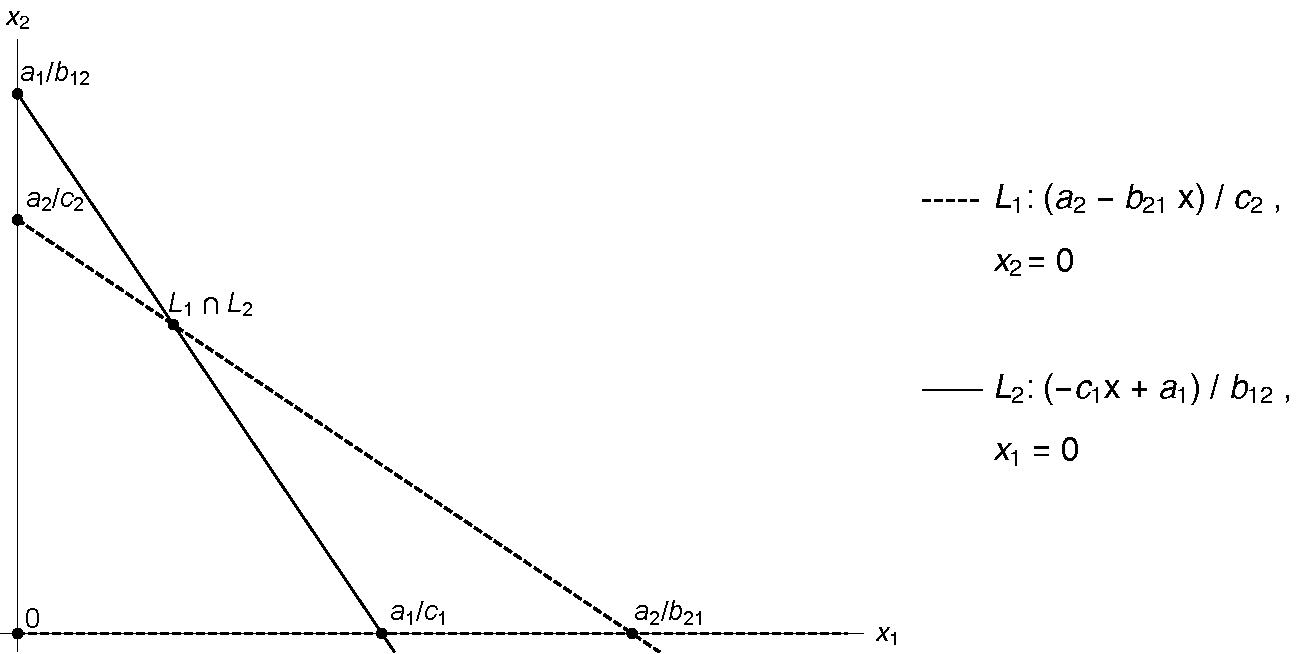
\includegraphics[width=\textwidth]{sep_1.pdf}
        \caption{Расположение прямых-сепаратрис, когда числитель и знаменатель положительные}
        \label{fig:sep_1}
    \end{figure}

    \begin{figure}
        \centering
        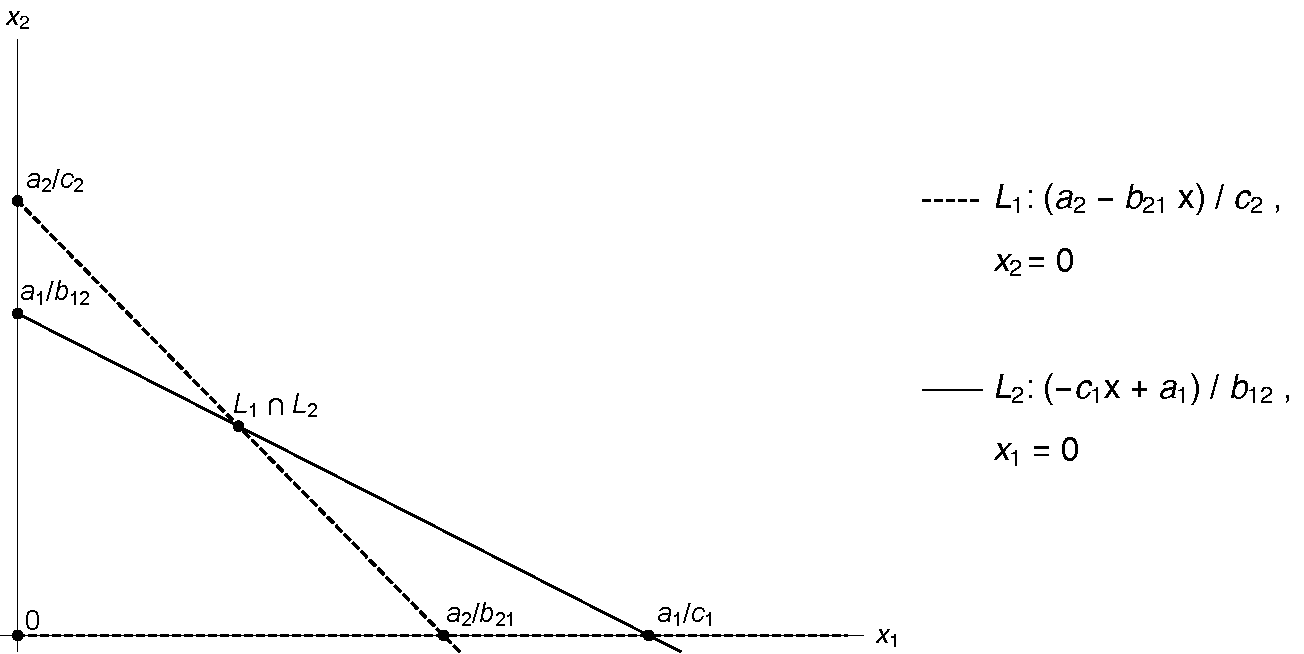
\includegraphics[width=\textwidth]{sep_2.pdf}
        \caption{Расположение прямых-сепаратрис, когда числитель и знаменатель отрицательные}
        \label{fig:sep_2}
    \end{figure}

    \pagebreak

    \section{Линеаризация системы в окрестности стационарных точкек}
    В общем виде линеаризованную систему можно представить в виде матрицы Якоби следющего вида: 
    \begin{equation}
        \label{jacobian}
        \mathbb{J} = 
            \begin{pmatrix}
                \dfrac{\partial{\dot x_1}}{\partial x_1}
                &
                \dfrac{\partial{\dot x_1}}{\partial x_2}
                \\[5mm]
                \dfrac{\partial{\dot x_2}}{\partial x_1}
                &
                \dfrac{\partial{\dot x_2}}{\partial x_2}
            \end{pmatrix}
        =
            \begin{pmatrix}
                a_1 - b_{12} x_2 - 2 c_1 x_1 & -b_{12} x_1
                \\
                -b_{21} x_2 & a_2 - b_{21} x_1 - 2c_2 x_2
            \end{pmatrix}\!.
    \end{equation}

    Линеаризуем систему в окрестности всех четырех стационарных точек:
    \[
        \mathbb{J}_{\rom 1} = 
                \begin{pmatrix}
                    a_1 & 0
                    \\
                    0   & a_2
                \end{pmatrix}\!,\quad
        \mathbb{J}_{\rom 2} = 
            \begin{pmatrix}
                -a_1 & -\dfrac{a_1 b_{12}}{c_1}
                \\[4mm]
                0   & \dfrac{a_2 c_1 - a_1 b_{21}}{c_1}
            \end{pmatrix}\!,\quad
        \mathbb{J}_{\rom 3} = 
            \begin{pmatrix}
                \dfrac{a_1 c_2 - b_{12} a_2}{c_2} & 0
                \\[4mm]
                -\dfrac{a_2 b_{21}}{c_2}          & -a_2
            \end{pmatrix}\!,
    \]

    \[
        \mathbb{J}_{\rom 4} = 
            \begin{pmatrix}
            \dfrac{c_1 (a_1 c_2 - a_2 b_{12})}{b_{12} b_{21} - c_1 c_2} & \dfrac{b_{12} (a_1 c_2 - a_2 b_{12})}{b_{12} b_{21} - c_1 c_2}
                \\[4mm]
                \dfrac{b_{21} (a_2 c_1 - a_1 b_{21})}{b_{12} b_{21} - c_1 c_2}   & \dfrac{c_2 (a_2 c_1 - a_1 b_{21})}{b_{12} b_{21} - c_1 c_2}
            \end{pmatrix}\!,
    \]
    \\
    и вспомним, что в зависимости от исходных параметров системы выполняется одно из двух условий(\refeq{positive}, \refeq{negative}), определящих типы этих точек. 

    \section{Фазовые портреты}
    Все стационарные точки являются простыми, поэтому их тип определяется собственными числами матриц $ \mathbb{J}_{\rom 1 - \rom 4}.$

    \subsection{Первый вариант параметров системы.}
    \begin{enumerate}
        \setlength\itemsep{0.5em}
        \item $ \lambda_1 = a_1 > 0,\ \lambda_2 = a_2 > 0 \Rightarrow $ точка $ (0, 0) $ --- неустойчивый узел;
    
        \item $ \lambda_1 = -a_1 < 0,\ \lambda_2 = \dfrac{a_2 c_1 - a_1 b_{21}}{c_1} > 0 \Rightarrow $ точка $ \left( \dfrac{a_1}{c_1}, 0 \right) $ --- седло;
        
        \item  $ \lambda_1 = \dfrac{a_1 c_2 - b_{12} a_2}{c_2} > 0,\ \lambda_2 = -a_2 < 0 \Rightarrow $ точка $ \left( 0, \dfrac{a_2}{c_2} \right) $ --- седло;
        
        \item Мне нужно расписывать все очень подробно или можно как-то сразу скзазать, что с.ч. отрицательные? ........ точка $ \left( \dfrac{a_1 c_2 - a_2 b_{12}}{c_1 c_2 - b_{12} b_{21}}, \dfrac{a_2 c_1 - a_1 b_{21}}{c_1 c_2 - b_{12} b_{21}} \right) $ --- устойчивый узел.
        \\
    \end{enumerate}

   Фазовый портрет с учетом условий (\refeq{positive}):
    \begin{figure}[h]
        \centering
        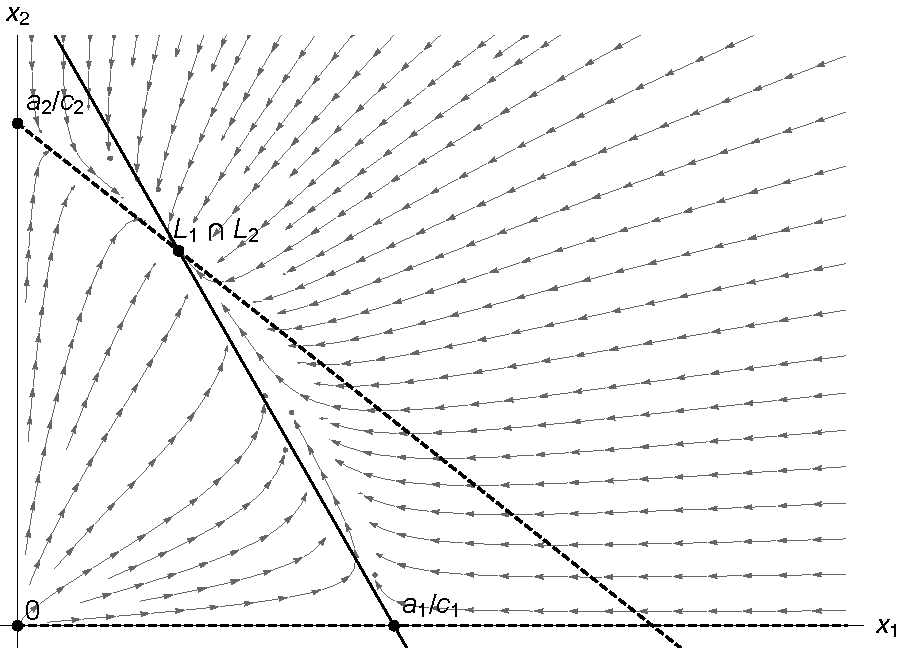
\includegraphics[width=0.75\textwidth]{phase_1.pdf}
        \caption{Характерный вид траекторий}
        \label{fig:phase_1}
    \end{figure}

    Из полученной картины можно сделать вывод, что сосуществование двух видов  гарантировано, потому что все траектории стремятся к $ 4^{\text{ой}} $ точке.

    \subsection{Второй вариант параметров системы}
    \begin{enumerate}
        \setlength\itemsep{0.5em}
        \item $ \lambda_1 = a_1 > 0,\ \lambda_2 = a_2 > 0 \Rightarrow $ точка $ (0, 0) $ --- неустойчивый узел;
    
        \item $ \lambda_1 = -a_1 < 0,\ \lambda_2 = \dfrac{a_2 c_1 - a_1 b_{21}}{c_1} < 0 \Rightarrow $ точка $ \left( \dfrac{a_1}{c_1}, 0 \right) $ --- устойчивый узел;
        
        \item  $ \lambda_1 = \dfrac{a_1 c_2 - b_{12} a_2}{c_2} < 0,\ \lambda_2 = -a_2 < 0 \Rightarrow $ точка $ \left( 0, \dfrac{a_2}{c_2} \right) $ --- устойчивый узел;
        
        \item $ \det \mathbb{J}_{\rom 4}\! < \!0 \Rightarrow$ собственные значения имеют разные знаки, а значит точка-пересечение сепаратрис $ \left( \dfrac{a_1 c_2 - a_2 b_{12}}{c_1 c_2 - b_{12} b_{21}}, \dfrac{a_2 c_1 - a_1 b_{21}}{c_1 c_2 - b_{12} b_{21}} \right) $ --- седло.
        \\
    \end{enumerate}

    Фазовые траектории с учетом условий (\refeq{negative}): 
    \begin{figure}[h]
        \centering
        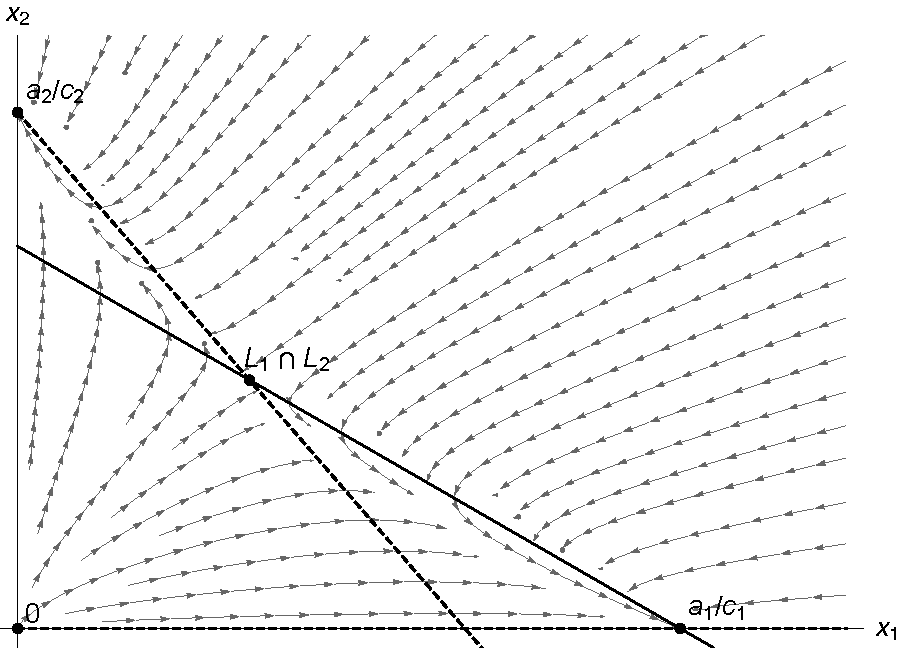
\includegraphics[width=0.75\textwidth]{phase_2.pdf}
        \caption{Характерный вид траекторий}
        \label{fig:phase_2}
    \end{figure}

    Таким образом, сосуществование двух конкурирующих видов крайне маловероятно. Большинство траекторий стремятся либо ко $ 2^{\text{ой}} $, либо к $ 3^{\text{ей}} $ точке. А они соответстуют вымиранию одного из видов.

    \section-{Заключение}
    Имея экспериментально выведенные коэфициенты размножения, а также коэфициенты межвидовой и внутривидовой конкуренции, мы можем построить модель взаимодействия между особями двух видов и понять, способны ли они сосуществовать или же один из них вымрет. Анализ особых точек (иными словами --- стационарных состояний) дает нам возможность построить график траекторий, чтобы определить, к какому из четырех стационарных состояний стремится система.

    \newpage

    \begin{thebibliography}{9}
        % \bibitem{Loyts} Лойцянский Л.\,Г. Механика жидкости и газа. М.: Дрофа, 2003. 846 с.

        \bibitem{Model} Ризниченко Г.\,Ю. Лекции по математическим моделям в биологии. --- 2-е изд. испр. и доп. --- М. --- Ижевск: Институт компьютерных исследований, НИЦ <<Регулярная и хаотическая динамика>>. 2010. 560 с.

        \bibitem{agafonov} Агафонов С.А., Герман А.Д., Муратова Т.В. Дифференциальные уравнения. М.: Изд-во МГТУ им. Н.Э. Баумана, 1997. 336 с.

        \bibitem{petrovsky} Петровский И.Г. Лекции по теории обыкновенных дифференциальных уравнений. М.: Наука. 1970. 280 с.

        \bibitem{pentryagin} Понтрягин Л.С. Обыкновенные дифференциальные уравнения. М.: Наука. 1970. 332 с.

        \bibitem{samarsky} Самарский А.А., Гулин А.В. Численные методы. М.: Наука: Физматлит, 1989. 416 с.

    \end{thebibliography}

    \end{document}

    http://mail.mce.su/material/mprac/1c.pdf

    https://www.yaklass.ru/p/biologia/obschie-biologicheskie-zakonomernosti/osnovy-ekologicheskikh-znanii-13908/bioticheskie-vzaimootnosheniia-organizmov-13910/re-ff2f6822-329f-48c8-a34f-7bf3a39b37ca



  \subsection{Окрестность точки, соответствующей вымиранию обоих видов}
    Рассмотрим стационарное состояние $ x_1 = 0,\ x_2 = 0 $. Подставим эти координаты в матрицу (\refeq{jacobian}) и получим:
    \begin{equation}
        \label{allDie}
        \mathbb{J}_{\rom 1} = 
            \begin{pmatrix}
                a_1 & 0
                \\
                0   & a_2
            \end{pmatrix}\!.
    \end{equation}

    По условию задачи коэфициенты $ a_1, a_2 $ строго положительные, поэтому корни $ \lambda_1 = a_1,\ \lambda_2 = a_2 $ также положительные. Таким образом, данная точка~--- неустойчивый узел.

    \subsection{Окрестность точки, соответствующей выживанию 1 вида}
    В окрестности точки, где $ x_1 = \frac{a_1}{c_1},\ x_2 = 0 $ матрица коэфициентов линеаризованной системы имеет вид:
    \begin{equation}
        \label{secondDie}
        \mathbb{J}_{\rom 2} = 
            \begin{pmatrix}
               -a_1 & -\dfrac{a_1 b_{12}}{c_1}
                \\[4mm]
                0   & \dfrac{a_2 c_1 - a_1 b_{21}}{c_1}
            \end{pmatrix}\!.
    \end{equation}
   
    Корни соответствующего характеристического уравнения: $ \lambda_1 = -a_1,\ \lambda_2 = $ \linebreak $ = \frac{a_2 c_1 - a_1 b_{21}}{c_1} $. Корень $ \lambda_1 $ отрицательный для $ \forall a_1 \in \mathbb{R} $. Рассмотрим корень $ \lambda_2 $ поподробнее:
    \begin{itemize}
        \item $ a_2 c_1 < a_1 b_{21} \Rightarrow \lambda_2 < 0, $ и данная точка является устойчивый узлом;
        \item $ a_2 c_1 > a_1 b_{21} \Rightarrow \lambda_2 > 0$ --- седло.
    \end{itemize}

    \subsection{Окрестность точки, соответствующей выживанию 2 вида}
    Рассмотрим следующее стационарное состояние, при котором $ x_1 = 0, $ \linebreak $ x_2 = \frac{a_2}{c_2} \colon$
    \begin{equation}
        \label{firstDie}
        \mathbb{J}_{\rom 3} = 
            \begin{pmatrix}
                \dfrac{a_1 c_2 - b_{12} a_2}{c_2} & 0
                \\[4mm]
                -\dfrac{a_2 b_{21}}{c_2}          & -a_2
            \end{pmatrix}\!.
    \end{equation}
    
    
    Тип этой точки определятся таким же образом, что и в предыдущем случае. Корень $ \lambda_2 = -a_2 $ всегда отрицательный. Корень $ \lambda_1 \colon$
    \begin{itemize}
        \item $ a_1 c_2 < a_2 b_{12} \Rightarrow \lambda_1 < 0, $ то есть данная точка --- устойчивый узел;
        \item $ a_1 c_2 > a_2 b_{12} \Rightarrow \lambda_1 > 0$ --- седло.
     \end{itemize}

    \subsection{Окрестность точки, соответствующей выживанию обоих видов}
     Наконец, рассмотрим последнее стационарное состояние:
     \begin{equation}
        \label{allLive}
        \mathbb{J}_{\rom 4} = 
            \begin{pmatrix}
               \dfrac{c_1 (a_1 c_2 - a_2 b_{12})}{b_{12} b_{21} - c_1 c_2} & \dfrac{b_{12} (a_1 c_2 - a_2 b_{12})}{b_{12} b_{21} - c_1 c_2}
                \\[4mm]
                \dfrac{b_{21} (a_2 c_1 - a_1 b_{21})}{b_{12} b_{21} - c_1 c_2}   & \dfrac{c_2 (a_2 c_1 - a_1 b_{21})}{b_{12} b_{21} - c_1 c_2}
            \end{pmatrix}\!.
    \end{equation}